\documentclass[12pt,A4paper,titlepage]{article}

%PAQUETES
\usepackage[spanish]{babel}
\usepackage[utf8]{inputenc} %Este paquete permite poner acentos directamente y ees
\usepackage{fontenc}
\usepackage{amsmath}
\usepackage{graphicx}%[pdftex]
\usepackage{graphicx, wrapfig}
\usepackage{fancyhdr}
\usepackage{anysize}
\usepackage{verbatim}
\usepackage{advdate}
\usepackage{colortbl}
\usepackage{amsmath}
\usepackage{amssymb}
\usepackage[dvips,final]{epsfig}
\usepackage{epstopdf}
\usepackage{hyperref}
\usepackage{enumitem}
\usepackage{siunitx}
\usepackage{sectsty}
\usepackage{array}
\usepackage{listings}
\usepackage{minted}
\usepackage{xcolor}
\marginsize {2.5cm}{2.5cm}{2.5cm}{2.5cm} %Primero margen izquierdo, Segundo margen derecho, Tercero margen superior, Cuarto margen inferior.
\usepackage{float}

%Línea de presentación
\usepackage{fancyhdr}
\pagestyle{fancy}
\fancyhf{}
\fancyhead[L]{Síntesis de Redes Activas - Trabajo Práctico Nº5}
\fancyfoot[L,RO]{\thepage}
\fancyfoot[LO]{}
\renewcommand{\footrulewidth}{0.1pt}


%CARATULA
\begin{document}

\begin{titlepage}

\thispagestyle{empty}


\begin{center}
    
\includegraphics[scale=0.4]{Imagenes Logo/unc_logo.png}
    
\includegraphics[scale=0.4]{Imagenes Logo/fcefyn_logo.jpg}
    \\[1cm]
    \vspace{5pt}
    \LARGE \textbf{Universidad Nacional de Córdoba}\\[0.5cm] 
    \large \textbf{Facultad de Ciencias Exactas, Físicas y Naturales} \\[0.5cm] 
    \large \textbf{Síntesis de Redes Activas}
    \\[0.5cm]
    \large \textbf{Trabajo Práctico Nº5}\\[0.5cm]
    \vspace{60pt}
    \begin{table}[!h]
    \centering
    \begin{tabular}{ll}
    \multicolumn{1}{c}{Nombre} & \multicolumn{1}{c}{DNI} \\
    Armida Abril & 41.436.299  \\
    Ruiz Tatur Manuel & 40.963.553
    \end{tabular}
    \end{table}
    \vspace{20pt}
    \begin{table}[!h]
    \centering
    \begin{tabular}{ll}
    \multicolumn{1}{c}{Docentes} & Ing. Pablo Ferreyra \\
     & Ing. Cesar Reale \\
     
    \end{tabular}
    \end{table}
    \vspace{20pt}
    \large 2023
\end{center}

\end{titlepage}

\newpage
\tableofcontents %Arma el índice

\newpage
\section{Introducción}
\hspace{1mm} En el presente informe, se describen las acciones llevadas a cabo en el marco de la quinta actividad práctica de laboratorio. Esta tarea implica la creación de un circuito de filtro fundamentado en amplificadores operacionales. Para avanzar en este proyecto, se llevaron a cabo cálculos analíticos respaldados por verificaciones en el software \texttt{Matlab}, así como mediciones realizadas mediante el software \texttt{Multisim} y \texttt{Python}.

\newpage
\section{Objetivos}
\hspace{1mm} En base a la planilla de requerimiento suministrada, se sintetiza un circuito en amplificadores operacionales que satisfaga esos requisitos.

\begin{figure}[!h] 
  \centering
  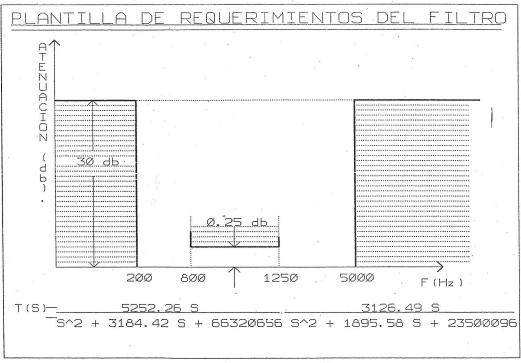
\includegraphics[scale=0.85]{Imagenes/Plantilla de requerimiento del filtro.png}
  \caption{\textit{Plantilla de requerimiento del filtro}}
\end{figure}


\hspace{1mm} En la mencionada plantilla, se especifica la síntesis de un filtro activo pasa banda que debe cumplir con requisitos específicos de respuesta en frecuencia. Estos requisitos incluyen lograr una atenuación en la banda de paso, ubicada entre \(800~Hz\) y \(1250~Hz\), que no exceda los \(0.25~dB\). Asimismo, se requiere que en las bandas de rechazo, comprendidas entre \(0~Hz\) y \(200~Hz\), y de \(5000~Hz\) en adelante, la atenuación sea al menos de \(30~dB\).

\bigskip
\hspace{1mm} Seguidamente, se debe:
\begin{itemize}[itemsep=1pt]
    \item Aproximar la función de atenuación mediante polinomios de Chebychev mediante Matlab.
    \item Sintetizar un circuito que satisfaga los requerimientos del punto anterior utilizando topologías bicuadráticas de realimentación positiva o negativa, a elección.
    \item Simular cada etapa y el filtro total.
    \item Calcular la sensibilidad de la frecuencia del polo de cada bicuadrática (\(\omega p\)) y el ancho de banda \(\frac{\omega p}{Qp}\).
    \item Analizar la peor desviación si todos los elementos tienen una tolerancia del 10\%.
    \item Realizar una simulación de Montecarlo de las desviaciones.
    \item Armar el circuito, medir experimentalmente las curvas de atenuación y desfasaje. Contractarlas con las predicciones teóricas y las simulaciones.
\end{itemize}

\newpage
\section{Marco teórico}
\hspace{1mm} Un filtro es cualquier dispositivo que modifica de un modo determinado una señal que pasa a través de él. Algunos autores sostienen la denominación de filtros para los dispositivos selectores de frecuencia, es decir, aquellos que 'dejan pasar' las señales presentes en ciertas bandas de frecuencia y las que 'bloquean' las señales de otras bandas.

\bigskip
\hspace{1mm} Se denominan filtros activos a los que utilizan elementos activos, como amplificadores y sus derivados. Estos filtros se modelan, partiendo de los requerimientos solicitados y proporcionan las características que tendrá el filtro en sí. Se los diferencia de los filtros pasivos ya que estos sólamente utilizan componentes pasivos. Para hallar la función de transferencia que cumpla con las condiciones requeridas se aplica la teoría de la aproximación, en la cual se pueden encontrar varios autores como Butterworth, Chebyshev, Cauer, entre otros.

\bigskip
\hspace{1mm} Mediante estas aproximaciones se obtiene entonces la función de transferencia que responderá a las solicitudes requeridas. Esta función final se expresa como una productoria de ecuaciones bicuadráticas con el fin de modelar individualmente cada una de ellas con diversas topologías obteniendo así los componentes físicos que corresponden a cada una de estas. Luego, se realiza una conexión en cascada de cada función. 

\bigskip
\hspace{1mm} En el presente trabajo práctico se utilizará un filtro pasa banda, el cual permite el paso de las frecuencias comprendidas entre dos frecuencias \(\omega_1 \) y \(\omega_2 \) con \(\omega_1 < \omega_2 \), denominadas frecuencia inferior de corte y frecuencia superior de corte, bloqueando las frecuencias restantes como se puede apreciar en la siguiente imagen. 

\begin{figure}[!h] 
  \centering
  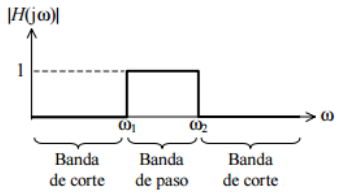
\includegraphics[scale=0.75]{Imagenes/Filtro pasa bandas.png}
  \caption{\textit{Filtro pasa banda}}
\end{figure}

\hspace{1mm} En lo que respecta a las topologías aplicadas para la síntesis de las funciones se pueden destacar tres de ellas:

\begin{itemize}[itemsep=1pt]
    \item Topología bicuadrática de realimentación positiva.
    \item Topología bicuadrática de realimentación negativa.
    \item Topología de 3 o 4 operacionales. 
\end{itemize}

\hspace{1mm} Por lo tanto, luego de seleccionar la forma en la que se resolverá el diseño del filtro, bastará sólo con realizar cálculos analíticos y adaptarlo al sistema pedido.

\newpage
\section{Desarrollo}

\hspace{1mm} En primer lugar se detallan los parámetros de entrada para luego poder obtener la función de transferencia por la aproximación de Chebyshev. A continuación se adjunta el código con los parámetros realizado en \texttt{Matlab}.

\begin{minted}[fontsize=\small,breakanywhere, breaklines]{Matlab}
    %% Parametros de entrada
    fp = [800 1250]     %Banda de paso [Hz]
    fs = [200 5000]     %Banda de rechazo [Hz]
    Wp = 2*pi*fp;       %Banda de Paso [rad/s]
    Ws = 2*pi*fs;       %Banda de Rechazo [rad/s]
    Ap = 0.25;          %Atenuacion maxima en Banda de Paso [dB]
    As = 30;            %Atenuacion minima en Banda de Rechazo [dB]
\end{minted}

\hspace{1mm} Es entonces que se procede a calcular la función de transferencia como se mencionó anteriormente. En esta instancia también se descompone la función en bicuadráticas y se realiza la implementación como pasa alto y pasa bajo.

\begin{minted}[fontsize=\small,breakanywhere, breaklines]{Matlab}
    %% Calculo de FT
    [n,Wp] = cheb1ord(Wp,Ws,Ap,As,'s');
    [num,den] = cheby1(n,Ap,Wp,'s');
    Filtro = tf(num,den)                %Funcion de transferencia calculada
    [sos,g] = tf2sos(num,den);          %Descomponemos en bicuadrativas
    
    %Implementacion como PasaAlto/PasaBajo
    PasaBajo = tf(2*g*sos(1,1:3),sos(1,4:6))
    PasaAlto = tf(1/2*sos(2,1:3),sos(2,4:6))
\end{minted}

\hspace{1mm} Los resultados que se obtuvieron son los siguientes.

\begin{figure}[!h] 
  \centering
  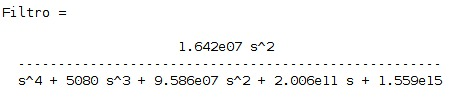
\includegraphics[scale=0.85]{Imagenes/Funcion de transferencia del filtro.png}
  \caption{\textit{Función de transferencia del filtro}}
\end{figure}

\begin{figure}[!h] 
  \centering
  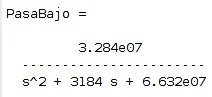
\includegraphics[scale=0.95]{Imagenes/Funcion de transferencia pasa bajo.png}
  \caption{\textit{Función de transferencia del filtro pasa bajo}}
\end{figure}

\begin{figure}[!h] 
  \centering
  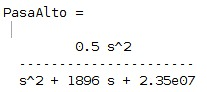
\includegraphics[scale=0.95]{Imagenes/Funcion de transferencia pasa alto.png}
  \caption{\textit{Función de transferencia del filtro pasa alto}}
\end{figure}


\newpage
\hspace{1mm} Por último, se detalla el diagrama de bode final donde se puede apreciar el filtro pasa banda.

\bigskip
\begin{figure}[!h] 
  \centering
  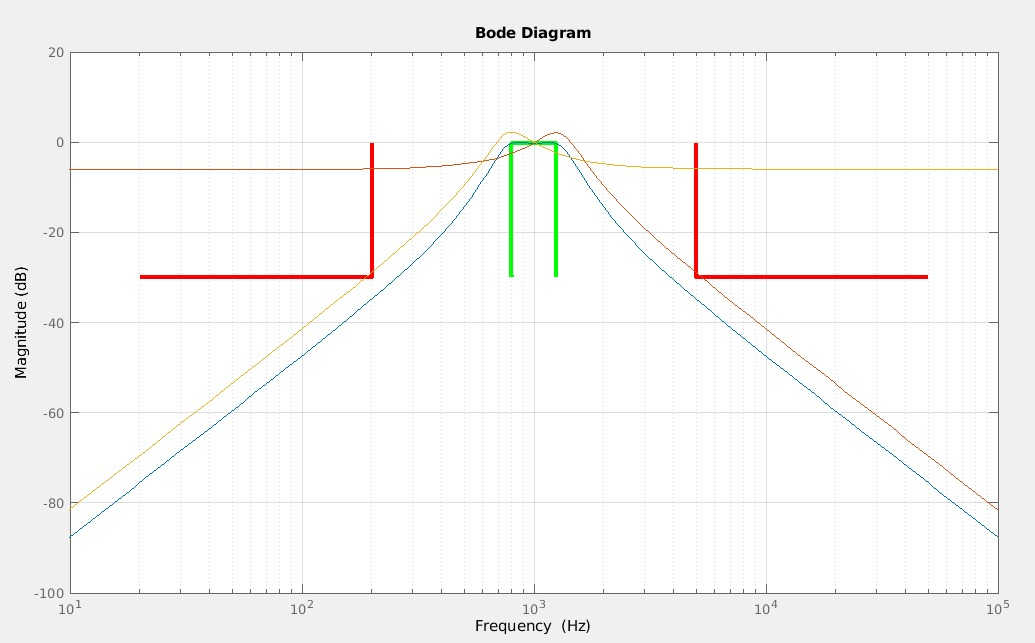
\includegraphics[scale=0.55]{Imagenes/DIagrama de bode.png}
  \caption{\textit{Diagrama de Bode}}
\end{figure}


\newpage
\subsection{Síntesis del circuito pasa banda}
\hspace{1mm} En esta etapa, se empleó el método de Sallen Key con una topología bicuadrática de realimentación positiva. Para ello, se implementó el siguiente circuito.

\begin{figure}[!h] 
  \centering
  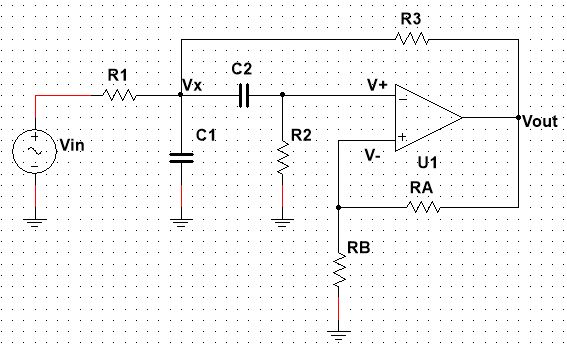
\includegraphics[scale=1]{Imagenes/Circuito de filtro general.png}
  \caption{\textit{Topología bicuadrática de realimentación positiva}}
\end{figure}

\hspace{1mm} El filtro pasa banda se representa con la siguiente ecuación.

\begin{equation}
    \frac{V_o}{V_{in}} = \frac{\frac{W_p}{Q_p} s}{s^2 + \frac{W_p}{Q_p} s + W_p^2}
\end{equation}

\bigskip
\hspace{1mm} Esta ecuación se utilizará como base para igualarla con la obtenida en MATLAB. A partir del circuito anterior, se deriva la ecuación de \(V^+\) para establecer una topología de realimentación positiva. De esta manera, se definen los distintos parámetros de la siguiente fórmula.

\begin{equation}
    A_v(s) = \frac{K . N_{FF}}{D - K . N_{FB}}
\end{equation}

\bigskip
\hspace{1mm} Para determinar los parámetros mencionados, se iniciará el desarrollo mediante el método de la matriz de nodos del siguiente circuito.

\newpage
\begin{figure}[!h] 
  \centering
  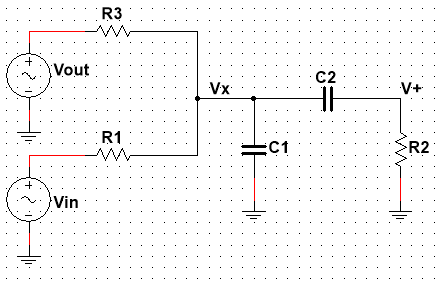
\includegraphics[scale=1]{Imagenes/Teoria de los nodos.png}
  \caption{\textit{Teoría de los nodos}}
\end{figure}

\bigskip
\hspace{1mm} Del mismo se obtiene la siguiente matriz de nodos.

\begin{figure}[!h] 
  \centering
  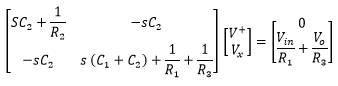
\includegraphics[scale=1]{Imagenes/Matriz de nodos.png}
  \caption{\textit{Matriz de los nodos}}
\end{figure}

\bigskip
\hspace{1mm} Siendo así la fórmula de \(V^+\) la siguiente.

\begin{figure}[!h] 
  \centering
  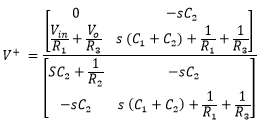
\includegraphics[scale=1]{Imagenes/Calculo deV+.png}
  \caption{\textit{Cálculo de \(V^+\)}}
\end{figure}

\newpage
\hspace{1mm} Si se resuelven las matrices resulta lo siguiente.

\begin{equation}
    V^+ = \frac{s (V_{in}\frac{C_2}{R_1} + V_o \frac{C_2}{R_3}) }{(s C_2 + \frac{1}{R_2}) (sC_1 + sC_2 + \frac{1}{R_1} + \frac{1}{R_3}) - s^2 C_2^2} 
\end{equation}

\bigskip
\hspace{1mm} Luego, al desarrollar la ecuación se tiene.

\begin{equation}
    V^+ = \frac{s (V_{in}\frac{C_2}{R_1} + V_o \frac{C_2}{R_3}) }{s^2 C_2 C_1 + s^2 C_2^2 + \frac{sC_2}{R_1} + \frac{sC_2}{R_3} + \frac{sC_1}{R_2} + \frac{sC_2}{R_2} + \frac{1}{R_1 R_2} + \frac{1}{R_3 R_2} - s^2 C_2^2} 
\end{equation}

\bigskip
\begin{equation}
    V^+ = \frac{s (V_{in}\frac{C_2}{R_1} + V_o \frac{C_2}{R_3}) }{s^2 C_2 C_1  + s(\frac{C_2}{R_1} + \frac{C_2}{R_3} + \frac{C_1}{R_2} + \frac{C_2}{R_2}) + \frac{1}{R_1 R_2} + \frac{1}{R_3 R_2}} 
\end{equation}

\bigskip
\begin{equation}
    V^+ = \frac{s (V_{in}\frac{C_2}{R_1} + V_o \frac{C_2}{R_3})}{s^2 C_2 C_1  + s((C_2(\frac{1}{R_1} + \frac{1}{R_2} + \frac{1}{R_3}) + \frac{C_1}{R_2})  + \frac{R_3 + R_1}{R_1 R_2 R_3}} 
\end{equation}

\bigskip
\hspace{1mm} Si se multiplica y divide por \(\frac{1}{C_2 C_1}\), se obtiene lo siguiente.

\bigskip
\begin{equation}
    V^+ = \frac{s (V_{in}\frac{1}{R_1 C_1} + V_o \frac{1}{R_3 C_1})}{s^2 + s((\frac{1}{C_1}(\frac{1}{R_1} + \frac{1}{R_2} + \frac{1}{R_3}) + \frac{1}{R_2 C_2})  + \frac{R_3 + R_1}{R_1 R_2 R_3 C_1 C_2}} 
\end{equation}

\bigskip
\hspace{1mm} Por lo tanto se pueden deducir los 3 parámetros fundamentales.

\begin{equation}
    N_{FF} = s \frac{1}{R_1 C_1}
\end{equation}

\begin{equation}
    N_{FB} = s \frac{1}{R_3 C_1}
\end{equation}

\begin{equation}
    D = s^2 + s (\frac{1}{C_1}(\frac{1}{R_1} + \frac{1}{R_2} + \frac{1}{R_3}) + \frac{1}{R_2 C_2}) + \frac{R_3 + R_1}{R_1 R_2 R_3 C_1 C_2}
\end{equation}

\bigskip
\hspace{1mm} Por lo que, reemplazando en la Ec.(2) resulta.

\begin{equation}
    A_v (s) = \frac{K . s \frac{1}{R_1 C_1}}{s^2 + s (\frac{1}{C_1}(\frac{1}{R_1} + \frac{1}{R_2} + \frac{1}{R_3}) + \frac{1}{R_2 C_2}) + \frac{R_3 + R_1}{R_1 R_2 R_3 C_1 C_2} - K. s\frac{1}{R_3 C_1}}
\end{equation}

\bigskip
\begin{equation}
    A_v (s) = \frac{ s \frac{K}{R_1 C_1}}{s^2 + s (\frac{1}{C_1}(\frac{1}{R_1} + \frac{1}{R_2} + \frac{1-K}{R_3}) + \frac{1}{R_2 C_2}) + \frac{R_3 + R_1}{R_1 R_2 R_3 C_1 C_2}}
\end{equation}

\bigskip
\hspace{1mm} Luego, se iguala la Ec.(12) con la Ec.(1) para poder determinar los siguientes coeficientes.

\begin{equation}
    W_p^2 = \frac{R_3 + R_1}{R_1 R_2 R_3 C_1 C_2}
\end{equation}

\begin{equation}
    \frac{W_p}{Q_p} = \frac{1}{C_1}(\frac{1}{R_1} + \frac{1}{R_2} + \frac{1-K}{R_3}) + \frac{1}{R_2 C_2}
\end{equation}

\bigskip
\hspace{1mm} Una aclaración importante es que se tomará como premisa que \(R_1 = R_2 = R_3 = 1\) y \(C_1 = C_2 = C\).

\bigskip
\hspace{1mm} Por lo tanto, se analizaron cada una de las funciones cuadráticas dando para cada caso los siguientes resultados.

\subsubsection{Caso del filtro pasa bajo}
\hspace{1mm} Para este caso se analizará la siguiente función bicuadrática.

\begin{figure}[!h] 
  \centering
  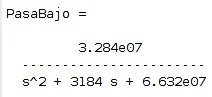
\includegraphics[scale=0.85]{Imagenes/Funcion de transferencia pasa bajo.png}
  \caption{\textit{Función de transferencia del filtro pasa bajo}}
\end{figure}

\hspace{1mm} Siendo entonces.

\begin{equation}
    W_p^2 = 66 320 656 = (\frac{R_3 + R_1}{R_1 R_2 R_3 C_1 C_2})^2
\end{equation}

\bigskip
 \hspace{1mm} Considerando las resistencias y capacitores mencionados anteriormente, la ecuación anterior se resume de la siguiente manera.
 
 \begin{equation}
     W_p^2 = 66 320 656 = \frac{2}{1[\Omega] C^2}
 \end{equation}

\begin{equation}
    W_p^2= 66 320 656 = \frac{2}{C^2}
\end{equation}

\bigskip
\hspace{1mm} Tomando raíz cuadrada a ambos miembros.

\begin{equation}
    W_p = 8 143.75 = \frac{\sqrt{2}}{C}
\end{equation}

\newpage
\hspace{1mm} Se despejó \(C\), obteniendo el siguiente resultado.

\begin{equation}
    C = \frac{\sqrt{2}}{8 143.75}
\end{equation}

\hspace{1mm} Siendo así.

\begin{equation}
    C = 174 [\mu F]
\end{equation}

\bigskip
\hspace{1mm} Los valores resultantes son \(R = 1 [\Omega]\) y \(C = 174 [\mu F]\). Es importante destacar que estos valores se escalan para que las unidades estén en rangos cotidianos, resultando en \(R = 1 [k\Omega]\) y \(C = 174 [nF]\).

\bigskip
\hspace{1mm} Igualando los términos de primer orden del denominador se tiene.

\bigskip
\begin{equation}
    \frac{W_p}{Q_p} = \frac{1}{C_1}(\frac{1}{R_1} + \frac{1}{R_2} + \frac{1-K}{R_3}) + \frac{1}{R_2 C_2}
\end{equation}

\bigskip
\hspace{1mm} Debido a las mismas consideraciones anteriores, la ecuación anterior se simplifica en.

\begin{equation}
    \frac{W_p}{Q_p} = \frac{1}{C}(\frac{1}{1} + \frac{1}{1} + \frac{1-K}{1}) + \frac{1}{1 C}
\end{equation}

\begin{equation}
    \frac{W_p}{Q_p} = \frac{4-K}{C}
\end{equation}

\hspace{1mm} Luego, como \(\frac{W_p}{Q_p} = 3184.42\), se despeja K y se obtiene lo siguiente.

\begin{equation}
    K = 4 - 3 184.42\cdot C 
\end{equation}

\bigskip
\hspace{1mm} Si se reemplaza con el valor de C antes de ser escaleado, el resultado de K es.
\begin{equation}
    K = 3.446
\end{equation}

\bigskip
\hspace{1mm} Como \(K = 1 - \frac{R_A}{R_B}\) se supuso una \(R_B = 1 [k\Omega]\) por lo tanto.

\begin{equation}
    R_A = (K - 1) \cdot R_B = 2.446[k \Omega]
\end{equation}

\bigskip
\hspace{1mm} Es así que el término del numerador resulta.

\begin{equation}
    \frac{K}{R.C} = \frac{3.446}{1[\Omega] 174[\mu F]} = 19 804.6
\end{equation}

\bigskip
\hspace{1mm} Finalmente, la función de transferencia del primer caso es de la siguiente manera.

\begin{equation}
    \boxed{
         T_1 (s) = \frac{19 804.6 s}{S^2 + 3 184.42 s + 6 632 656}
    }
\end{equation}

\newpage
%filtro pasa alto
\subsubsection{Caso del filtro pasa alto}
\hspace{1mm} Para este caso se analizará la siguiente función bicuadrática.

\begin{figure}[!h] 
  \centering
  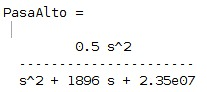
\includegraphics[scale=0.85]{Imagenes/Funcion de transferencia pasa alto.png}
  \caption{\textit{Función de transferencia del filtro pasa alto}}
\end{figure}

\hspace{1mm} Si se realiza el mismo procedimiento que para el caso anterior se consigue el valor de \(W_p ^2 \).

\begin{equation}
    W_p^2 = 23 500 000 = (\frac{R_3 + R_1}{R_1 R_2 R_3 C_1 C_2})^2
\end{equation}

\bigskip
 \hspace{1mm} Así mismo, si se toman las consideraciones de las resistencias y capacitores, la ecuación anterior se resume en la siguiente.
 
 \begin{equation}
     W_p^2 = 23 500 000 = \frac{2}{1[\Omega] C^2}
 \end{equation}

\begin{equation}
    W_p^2= 23 500 000 = \frac{2}{C^2}
\end{equation}

\bigskip
\hspace{1mm} Tomando raíz cuadrada a ambos miembros.

\begin{equation}
    W_p = 4 847.68 = \frac{\sqrt{2}}{C}
\end{equation}

%desde aca
\bigskip
\hspace{1mm} Se despeja C con lo que resulta.

\begin{equation}
    C = \frac{\sqrt{2}}{4 847.68}
\end{equation}

\hspace{1mm} Siendo así.

\begin{equation}
    C = 291.73 [\mu F]
\end{equation}

\bigskip
\hspace{1mm} Es entonces que los valores obtenidos son \(R=1 [\Omega]\) y \(C = 291.73 [\mu F]\). Observar que los mismos fueron escalados para que las escalas de las unidades se encuentren en sus valores cotidianos. Es así que los valores finales son \(R = 1 [k\Omega]\) y \(C = 291.73 [nF]\).

\newpage
\hspace{1mm} Igualando los términos de primer orden del denominador se tiene.

\begin{equation}
    \frac{W_p}{Q_p} = \frac{1}{C_1}(\frac{1}{R_1} + \frac{1}{R_2} + \frac{1-K}{R_3}) + \frac{1}{R_2 C_2}
\end{equation}

\bigskip
\hspace{1mm} Debido a las mismas consideraciones anteriores, la ecuación anterior se simplifica en.

\begin{equation}
    \frac{W_p}{Q_p} = \frac{1}{C}(\frac{1}{1} + \frac{1}{1} + \frac{1-K}{1}) + \frac{1}{1 C}
\end{equation}

\begin{equation}
    \frac{W_p}{Q_p} = \frac{4-K}{C}
\end{equation}

\hspace{1mm} Luego, como \(\frac{W_p}{Q_p} = 1 896\), se despeja K y se obtiene lo siguiente.

\begin{equation}
    K = 4 - 1 896\cdot C 
\end{equation}

\bigskip
\hspace{1mm} Si se reemplaza con el valor de C antes de ser escaleado, el resultado de K es.
\begin{equation}
    K = 3.447
\end{equation}

\bigskip
\hspace{1mm} Como \(K = 1 - \frac{R_A'}{R_B'}\) se supuso una \(R_B' = 1 [k\Omega]\) por lo tanto.

\begin{equation}
    R_A' = (K - 1) \cdot R_B' = 2.447[k \Omega]
\end{equation}

\bigskip
\hspace{1mm} Es así que el término del numerador resulta.

\begin{equation}
    \frac{K}{R.C} = \frac{3.447}{1[\Omega] 291.73[\mu F]} = 11 815.7
\end{equation}

\bigskip
\hspace{1mm} Finalmente, la función de transferencia del primer caso es de la siguiente manera.

\begin{equation}
    \boxed{
    T_2 (s) = \frac{11 815.7 s}{S^2 + 1 896 s + 23 500 000}
    }
\end{equation}

\newpage
\subsection{Calculo de la Atenuación}
\hspace{1mm} Se procedió a calcular la atenuación del circuito completo multiplicando las dos funciones obtenidas, dando como resultado la siguiente función de transferencia.

\begin{equation}
    T (s) = T_1 \cdot T_2 = \frac{19 804.6 s}{S^2 + 3 184.42 s + 6 632 656} \cdot \frac{11 815.7 s}{S^2 + 1 896 s + 23 500 000}
\end{equation}

\hspace{1mm} Por lo tanto.

\begin{equation}
    T (s) = \frac{234 005 212.2 \hspace{1mm} s^4}{s^4 + 5080 s^3 + 9.586 \cdot 10^7 s^2 + 2.006 \cdot 10^11 s + 1.559 \cdot 10^15}
\end{equation}

\begin{equation}
   T(s) = \frac{1.642 \cdot 10^7 \hspace{1mm} s^2}{s^4 + 5080 s^3 + 9.586 \cdot 10^7 s^2 + 2.006 \cdot 10^11 s + 1.559 \cdot 10^15}
\end{equation}

\bigskip
\hspace{1mm} Estas presentan una diferencia en las ganancias. A raíz de esta disparidad, se debe atenuar la entrada mediante la implementación de un divisor resistivo, como se ilustra en la siguiente figura.

\begin{figure}[!h] 
  \centering
  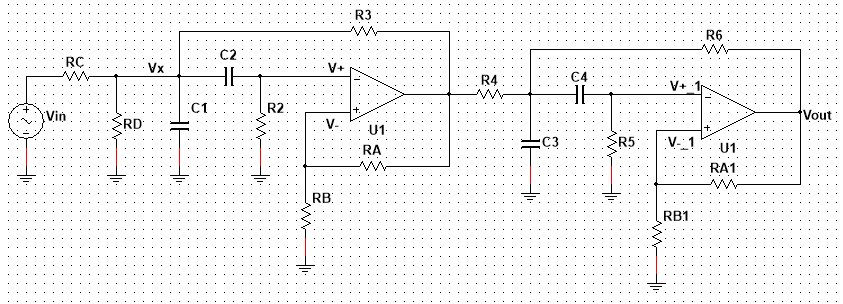
\includegraphics[scale=0.75]{Imagenes/Circuito atenuado.png}
  \caption{\textit{Circuito atenuado}}
\end{figure}


\hspace{1mm} Se deben calcular las resistencias \(R_C\) y \(R_D\). Para esto, se inicia calculando la ganancia del atenuador, \(\alpha\), con la siguiente fórmula.

\begin{equation}
    \alpha = \frac{16 420 000}{234 005 212.2} = 0.07
\end{equation}

\bigskip
\hspace{1mm} Posteriormente, se tienen dos ecuaciones fundamentales para determinar los valores de \(R_C\) y \(R_D\). Por un lado, al realizar el equivalente de Thévenin, se obtiene \(R_{T} = R_1\), que representa el paralelo entre \(R_C\) y \(R_D\). Por otro lado, la ganancia del atenuador puede igualarse a un divisor resistivo entre \(R_C\) y \(R_D\). De esta manera, se obtiene lo siguiente.

\begin{equation}
    R_1 = \frac{R_C R_D}{R_C + R_D}
\end{equation}

\begin{equation}
    \alpha = \frac{R_D}{R_C + R_D}
\end{equation}

\bigskip
\hspace{1mm} Entonces, si se reemplaza \(\alpha \) en la Ec.(30), se tiene.

\begin{equation*}
    R_1=R_C\alpha 
\end{equation*}

\hspace{1mm} Por lo que, 

\begin{equation}
    R_C = \frac{R_1}{\alpha}
\end{equation}

\hspace{1mm} Reemplazando por los valores de \(R_1\) y \(\alpha\) se tiene.

\bigskip
\begin{equation}
    R_C = \frac{R_1}{\alpha} = \frac{1[K\Omega]}{0.07}
\end{equation}

\begin{equation}
    \boxed{
    R_C = = 14.28[K\Omega]
    }
\end{equation}

\bigskip
\hspace{1mm} Luego, para obtener el valor de \(R_D\) se despeja dicho valor de la Ec. (46) resulta.

\begin{equation}
    R_D = R_C \hspace{1mm} (\frac{\alpha}{1 - \alpha})
\end{equation}

\bigskip
\hspace{1mm} Dando como resultado una.

\begin{equation}
    \boxed{
        R_D = 33.32[k \Omega] 
    }   
\end{equation}

\newpage
\subsection{Cálculo de la Sensibilidad}
\hspace{1mm} Para el cálculo de la sensibilidad de la frecuencia del polo (\(\omega_p\)) y el ancho de banda (\(\omega_p/Q_p\)), se toma de la ecuación principal la deducción de \(\omega_p\).
\begin{equation}
    \omega_p=\frac{\sqrt{(R_1+R_3)}}{\sqrt{R_1*R_2*R_3*C_1*C_2}}\cong \frac{\sqrt{2}}{\sqrt{R_1*R_2*C_1*C_2}}
\end{equation}

\bigskip
\hspace{1mm} Luego, para el ancho de banda se tiene.

\bigskip
\begin{equation}
    \frac{\omega_p}{Q_p}=\frac{1}{R_1C_1}+\frac{1}{R_2C_2}+\frac{1}{R_2C_1}+\frac{1-K}{R_3C_1}
\end{equation}

\bigskip
\hspace{1mm} Por lo tanto, se define la sensibilidad de \(\omega_p \) respecto de una R de la red como:
\begin{equation}
    S_R^{\omega_p} = \lim_{\Delta R \rightarrow 0} \frac{\frac{\Delta \omega_p}{\omega_p}}{\frac{\Delta R}{R}} =\frac{R}{\omega_p}\cdot \frac{\partial \omega_p}{\partial R}
\end{equation}

\hspace{1mm} Y, de forma análoga, la sensibilidad de  \(\omega_p \) respecto de un C de la red como:
\begin{equation}
    S_C^{\omega_p} = \lim_{\Delta C \rightarrow 0} \frac{\frac{\Delta \omega_p}{\omega_p}}{\frac{\Delta C}{C}} =\frac{C}{\omega_p}\cdot \frac{\partial \omega_p}{\partial C}
\end{equation}

\hspace{1mm} Se realiza una tabla con las sensibilidades correspondientes.

\begin{figure}[!h] 
  \centering
  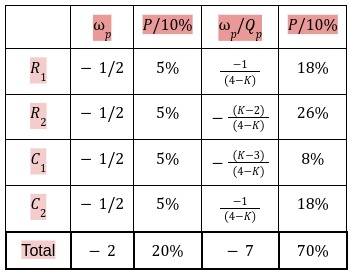
\includegraphics[scale=0.95]{Imagenes/Tabla con sensibilidades.png}
  \caption{\textit{Tabla de sensibilidades}}
\end{figure}

\newpage
\section{Resultados}
\subsection{Análisis de simulación de Montecarlo}
\hspace{1mm} Para el siguiente estudio se plantea una distribución Gaussiana de los componentes pasivos que conforman el filtro que se pretende sintetizar. A diferencia del estudio de la sensibilidad realizado anteriormente, donde se consideró el peor caso de las tolerancias de los componentes actuando de manera simultánea, en esta parte se tomará la distribución normal de los componentes, la cual no tiene por qué ser el peor de los casos. Es entonces que se plantea una distribución estadística del posible valor de la frecuencia del polo de cada etapa \(\omega_p\) o, del ancho de banda correspondiente \(\omega_p/Q_p\).

\bigskip
\hspace{1mm} Por lo tanto, el siguiente estudio se realizará en Python. Se generarán valores aleatorios para de resistores y capacitores, cuya dispersión corresponde a la tolerancia de los mismos (para este estudio se considera una tolerancia del \(10\%\) ).

\bigskip
\hspace{1mm} Para los valores aleatorios de capacitores y resistores, se plantea una distribución normal. A partir de estos resultados se puede hallar la media y el desvío estándar de cada componente. De forma análoga, si se emplean las ecuaciones encontradas para \(\omega_p\) y \(\omega_p/Q_p\), se pueden hallar diversos valores para los mismos. Es entonces que para estos también se plantea una distribución normal consideranco la media y el desvío estándar. A continuación se detallan los distintos casos luego de realizar 100 iteraciones en cada uno. 

\subsubsection{Resistencia}

\hspace{1mm} El análisis de esta parte se realizará una sola vez para las dos etapas (filtro pasa bajos y filtro pasa altos), ya que el valor de las resistencias en ambas etapas es el mismo. A continuación se tiene el gráfico de la distribución normal de los resistores para ambas etapas y los resultados de la media y el desvío.

\begin{figure}[!h] 
  \centering
  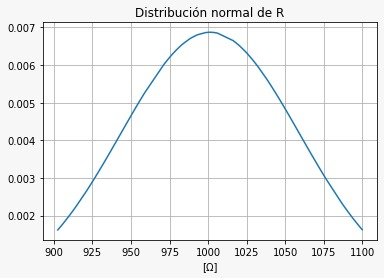
\includegraphics[scale=0.55]{Imagenes/Distribución normal de R.png}
  \caption{\textit{Distribución normal de R}}
\end{figure}

\begin{equation}
    \boxed{Media = 1001.29 [\Omega]}     
\end{equation}

\begin{equation}
    \boxed{Desvio = 58.06 [\Omega]}
\end{equation}

\bigskip

\newpage
\subsubsection{Capacitores - Etapa del fitro pasa bajo}
\hspace{1mm} Los resultados de la simulación son los siguientes.

\begin{equation}
   \boxed{ Media = 173.54 [nF] }    
\end{equation}

\begin{equation}
    \boxed{Desvio = 10.26 [nF]}
\end{equation} 

\begin{figure}[!h] 
  \centering
  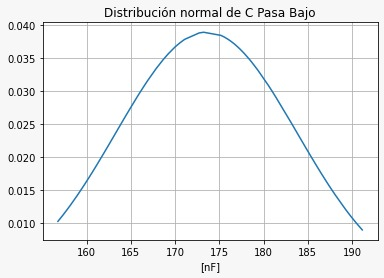
\includegraphics[scale=0.7]{Imagenes/Distribución normal de C pasa bajo.png}
  \caption{\textit{Distribución normal de \(C_1\) pasa bajo}}
\end{figure}

\subsubsection{Capacitores - Etapa del fitro pasa alto}
\hspace{1mm} Los resultados de la simulación son los siguientes.

\begin{equation}
    \boxed{Media = 292.13 [nF]}    
\end{equation}

\begin{equation}
    \boxed{Media = 292.13 [nF]}
\end{equation}

\begin{figure}[!h] 
  \centering
  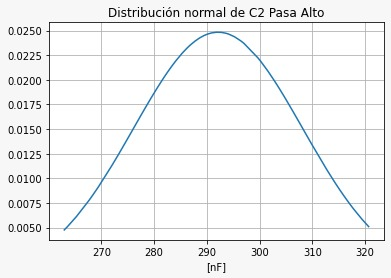
\includegraphics[scale=0.7]{Imagenes/Distribución normal de C2 pasa alto.png}
  \caption{\textit{Distribución normal de \(C_2\) pasa alto}}
\end{figure}

\newpage
\subsubsection{Frecuencia del polo - Etapa del fitro pasa bajo}
\hspace{1mm} Los resultados de la simulación son los siguientes.

\begin{equation}
    \boxed{Media = 8133.44 [rad/seg]}   
\end{equation}

\begin{equation}
    \boxed{Desvio = 460 [rad/seg]}
\end{equation}

\begin{figure}[!h] 
  \centering
  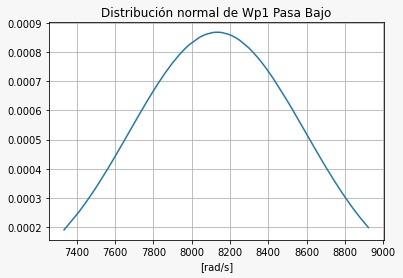
\includegraphics[scale=0.7]{Imagenes/Distribución normal de Wp1 pasa bajo.png}
  \caption{\textit{Distribución normal de \(\omega_{p1}\) pasa bajo}}
\end{figure}

\subsubsection{Frecuencia del polo - Etapa del fitro pasa alto}
\hspace{1mm} Los resultados de la simulación son los siguientes.

\begin{equation}
    \boxed{Media = 4847.12 [rad/seg]}     
\end{equation}

\begin{equation}
    \boxed{Desvio = 251.5 [rad/seg]}
\end{equation}

\begin{figure}[!h] 
  \centering
  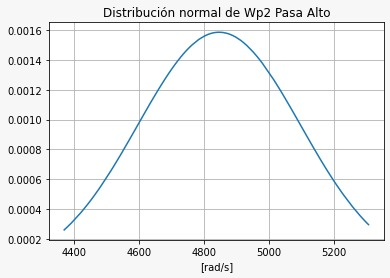
\includegraphics[scale=0.7]{Imagenes/Distribución normal de Wp2 pasa alto.png}
  \caption{\textit{Distribución normal de \(\omega_{p2}\) pasa alto}}
\end{figure}

\newpage
\subsubsection{Ancho de banda - Etapa del fitro pasa bajo}
\hspace{1mm} Los resultados de la simulación son los siguientes.

\begin{equation}
    \boxed{Media = 3167.21 [rad/seg] }    
\end{equation}

\begin{equation}
    \boxed{Desvio = 170 [rad/seg]}
\end{equation}

\begin{figure}[!h] 
  \centering
  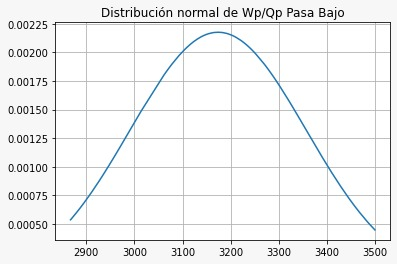
\includegraphics[scale=0.7]{Imagenes/Distribución normal de Wp1Qp1 pasa bajo.png}
  \caption{\textit{Distribución normal de \(\ \frac{W_{p1}}{Q_{p1}}\) pasa bajo}}
\end{figure}

\subsubsection{Ancho de banda - Etapa del fitro pasa alto}
\hspace{1mm} Los resultados de la simulación son los siguientes.

\begin{equation}
    \boxed{Media = 1888.17 [rad/seg]}     
\end{equation}

\begin{equation}
    \boxed{Desvio = 102.17 [rad/seg]}
\end{equation}

\begin{figure}[!h] 
  \centering
  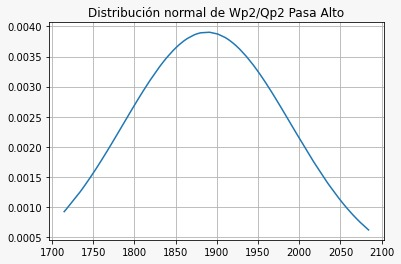
\includegraphics[scale=0.7]{Imagenes/Distribución normal de Wp2Qp2 pasa alto.png}
  \caption{\textit{Distribución normal de \(\ \frac{W_{p2}}{Q_{p2}}\) pasa alto}}
\end{figure}


\section{Simulaciones}
\subsection{Circuito simulado}
\hspace{1mm} En esta sección del trabajo práctico se presentan los resultados obtenidos del armado del circuito del filtro en simulación. Algunos valores fueron ajustados de manera proporcional sin alterar las condiciones propuestas para el sistema. Este ajuste se llevó a cabo con el objetivo de adecuar los valores calculados a componentes comerciales estándar.

\bigskip
\hspace{1mm} A continuación se adjunta una imágen del circuito simulado.

\begin{figure}[!h] 
  \centering
  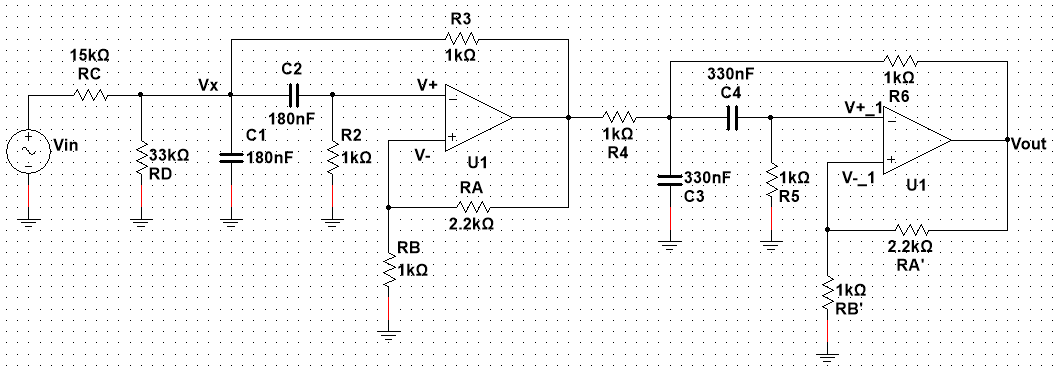
\includegraphics[scale=0.55]{Imagenes/Circuito completo real.png}
  \caption{\textit{Circuito completo real}}
\end{figure}

\hspace{1mm} Por último, se realiza una tabla comparativa para los valores simulados y requeridos. 

\begin{figure}[!h] 
  \centering
  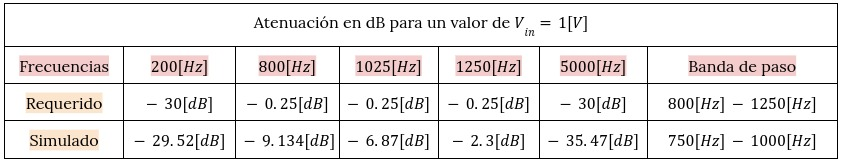
\includegraphics[scale=0.70]{Imagenes/Tabla comparativa.png}
  \caption{\textit{Tabla comparativa}}
\end{figure}

\bigskip
\hspace{1mm} Se puede observar que los valores medidos difieren ligeramente de los valores requeridos. Esta variación se debe a que los componentes tienen tolerancias que pueden afectar su comportamiento. En consecuencia, no se logró obtener un filtro ideal, pero se logró una aproximación bastante cercana.

\bigskip
\hspace{1mm} Mediante la simulación en Multisim, se generó el diagrama de Bode, donde se realizaron mediciones en las frecuencias requeridas, obteniendo los siguientes resultados.

\newpage
\hspace{1mm} Para el caso en que la frecuencia es \(200 [Hz]\).

\begin{figure}[!h] 
  \centering
  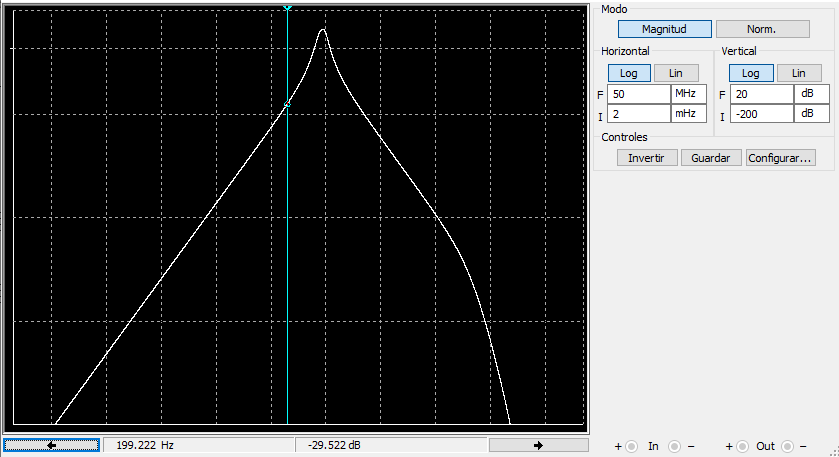
\includegraphics[scale=0.7]{Imagenes/Diagrama de bode 200Hz.png}
  \caption{\textit{Diagrama de bode en \(200 [Hz]\)}}
\end{figure}

\hspace{1mm} Para el caso donde la frecuencia es \(800 [Hz]\).

\begin{figure}[!h] 
  \centering
  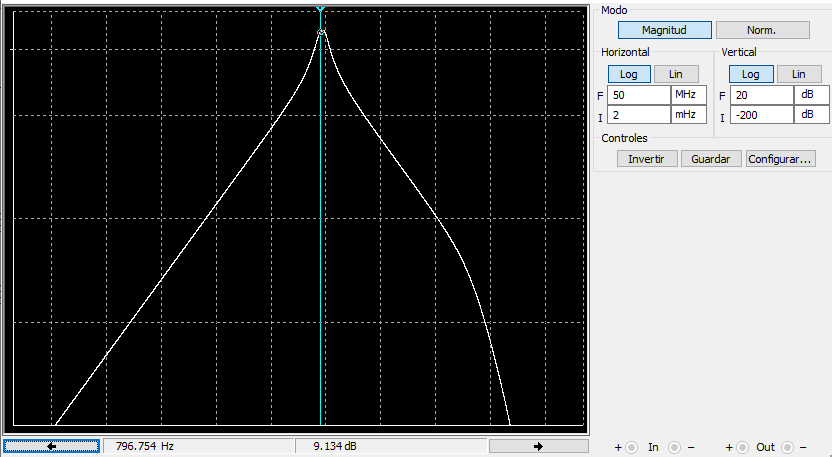
\includegraphics[scale=0.7]{Imagenes/Diagrama de bode 800Hz.png}
  \caption{\textit{Diagrama de bode en \(800 [Hz]\)}}
\end{figure}

\newpage
\hspace{1mm} Para el caso donde la frecuencia es \(1025 [Hz]\).

\begin{figure}[!h] 
  \centering
  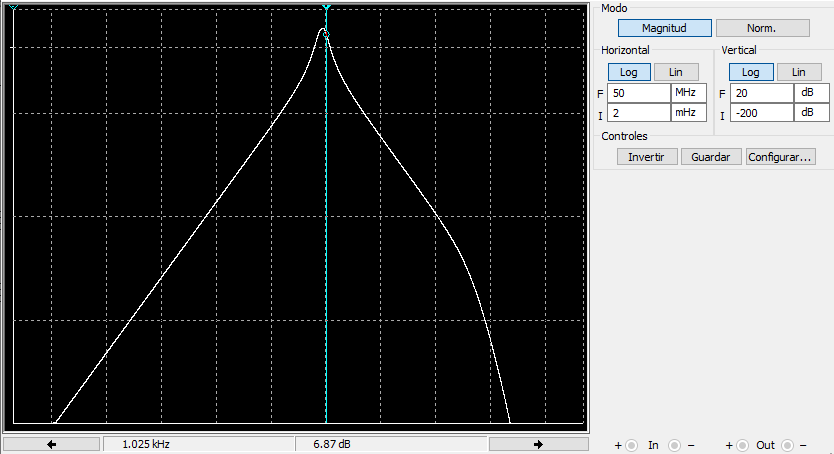
\includegraphics[scale=0.7]{Imagenes/Diagrama de bode 1025 Hz.png}
  \caption{\textit{Diagrama de bode en \(1025 [Hz]\)}}
\end{figure}

\hspace{1mm} Para el caso donde la frecuencia es \(1250 [Hz]\).

\begin{figure}[!h] 
  \centering
  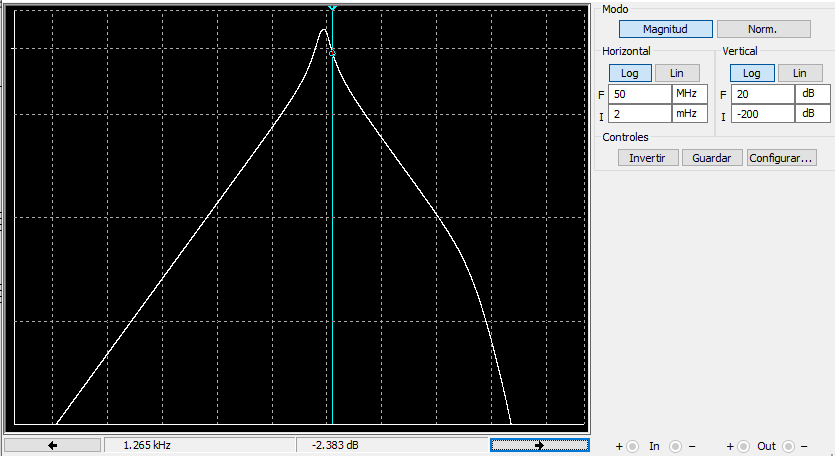
\includegraphics[scale=0.7]{Imagenes/Diagrama de bode 1250Hz.png}
  \caption{\textit{Diagrama de bode en \(1250 [Hz]\)}}
\end{figure}

\newpage
\hspace{1mm} Para el caso donde la frecuencia es \(5000 [Hz]\).

\begin{figure}[!h] 
  \centering
  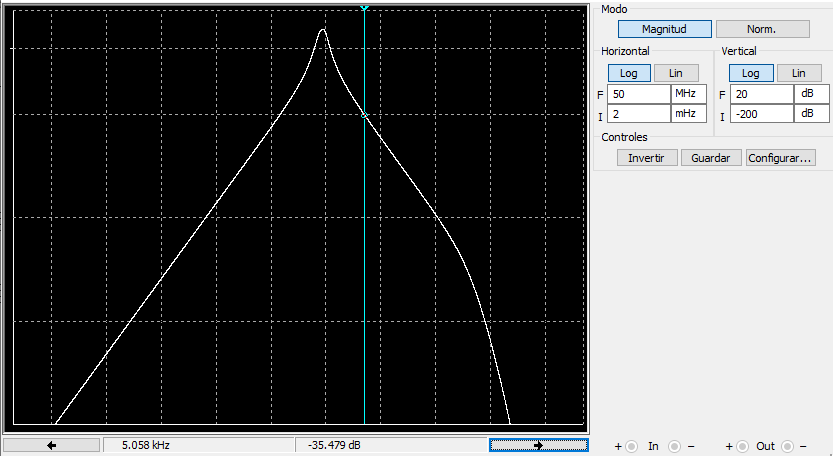
\includegraphics[scale=0.7]{Imagenes/Diagrama de bode 5000Hz.png}
  \caption{\textit{Diagrama de bode en \(5000 [Hz]\)}}
\end{figure}

\bigskip
\hspace{1mm} En conclusión, los resultados obtenidos indican que se logró desarrollar un filtro que cumple de manera confiable con las especificaciones establecidas.

\newpage
\section{Anexos}
\hspace{1mm} En esta sección se adjuntan los enlaces donde se encuentran los códigos y circuitos relacionados con el trabajo práctico, desarrollados en Python, MATLAB y Multisim.

\begin{itemize}
  \item Código de Python: \href{https://drive.google.com/drive/u/1/folders/1fn2AohxBO8u0CoIdvzcblCPVYjSHX1o6}{Enlace al código}
  \item Código de MATLAB: \href{https://drive.google.com/drive/u/1/folders/1jXmiKLY8pMCHEQzc57ifM0zqxy9C7B6I}{Enlace al código}
  \item Circuito en Multisim: \href{https://drive.google.com/drive/u/1/folders/1w0o-CqxwTwL3AFiesvhs8fyIltAos4nD}{Enlace al circuito}
\end{itemize}



\end{document}
